Immediately following the Big Bang, the Universe was primarily composed of a hot plasma of fundamental particles. In its early state, it was  too hot and dense to form the atoms that form the complex structures that we observe today. Photons that were emitted during this early period scattered off free particles, leaving the Universe opaque to electromagnetic radiation. This lasted until roughly 400,000 years after the Big Bang, at which time the Universe had expanded and cooled sufficiently for electrons to bind to atomic nuclei forming the first atoms of hydrogen and helium. Once formed, photons were able to freely propagate through the intergalactic medium (IGM). Today, we observe this cosmic microwave background radiation (CMB).

\begin{figure}[th]
	\centering
	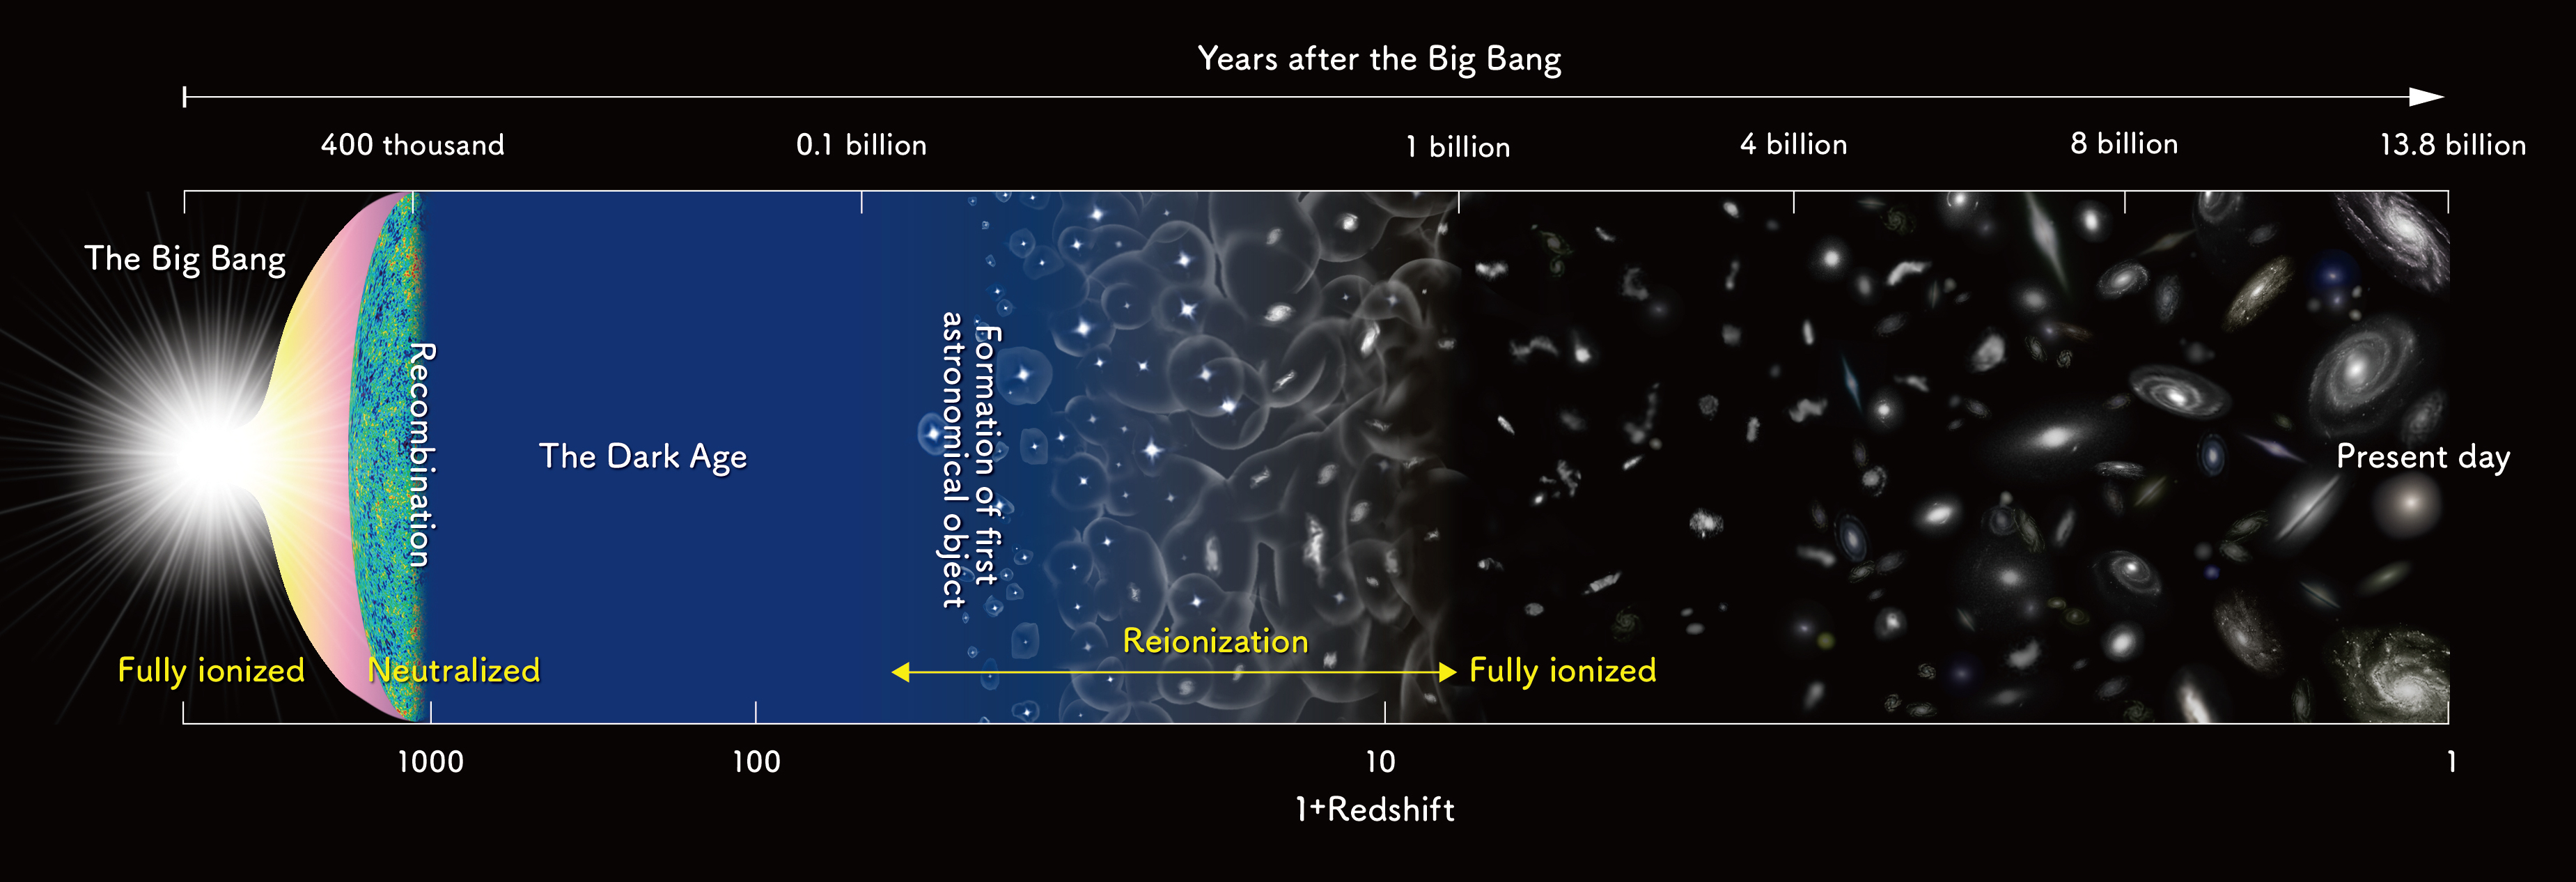
\includegraphics[width=1.0\textwidth]{intro/reionization.png}
	\caption[Epoch of Reionization Timeline]{Timeline of the history of the universe from its formation (left) to present day (right).}
	\label{fig:timeline}
\end{figure}

Following this recombination of matter, the universe was largely neutral and stationary.
Stars had not yet formed and the only emission detectable from this period originated
from neutral hydrogen. This period, called the Cosmic Dark Ages, lasted until roughly a few hundred millions after the Big Bang,
at which time the first luminous sources came into existence. Emitting ultraviolet (UV)
radiation, these first stars and galaxies began ionizing the neutral gas around them.
This period of time between the emergence of the first luminous sources and the
ionization of the neutral gas between them, named the Epoch of Reionization (EoR),
is believed to have lasted until around a billion years after the Big Bang.

Today, galaxies . Studying the EoR provides us the opportunity to establish a
bridge between the CMB and the structures we observe today, as well as provide
insight to what the first luminous objects were like and how they formed.
